\section{Quantum GIS 1.0}
\pagenumbering{arabic}
\setcounter{page}{1}

Quantum GIS (QGIS) is a user friendly Geographic Information System (GIS).
It is written in C++ and Python with a Qt4 based GUI. It is licensed under the
GNU General Public License (GPL) and an official project of the Open Source
Geospatial Foundation (OSGeo). The current stable version 1.0 was released in
January 2009. 

\minisec{History}

The QGIS project started in February of 2002, with the first release in June
of the same year. The initial goal was to create a viewer for PostGIS data
that ran on GNU/Linux. From those beginnings, QGIS has become a true
cross-platform application that runs on all major versions of Unix,
GNU/Linux, as well as Mac OSX and MS Windows. It supports numerous vector,
raster, and database formats and provides a wide variety of core and external
geoprocessing functionalities.

\subsection{QGIS Open Source Community}

The QGIS project is the work of a group of dedicated developers,
translators, documenters, release helpers, bug reporters, and promoters. Their 
contributions are mainly on a voluntary basis, except in a few cases where 
contributors are able to contribute to QGIS as part of their daily work. QGIS 
is managed by the Project Steering Committee (PSC), a five member committee
providing technical guidance, community liaison, release management, and
financial/marketing activities. The work of the QGIS project process is
spread between numerous people who each have a specific area of
responsibility, and ad-hoc contributors.

These volunteers together with a large number of users make up the
world-wide QGIS community. Over time their efforts have resulted in a comprehensive,
valuable and useful code and documentation base which is free for everyone 
to use and improve upon.

\begin{figure}[h]
   \begin{center}
   \caption{QGIS Community Map}\label{fig:community-map}\smallskip
   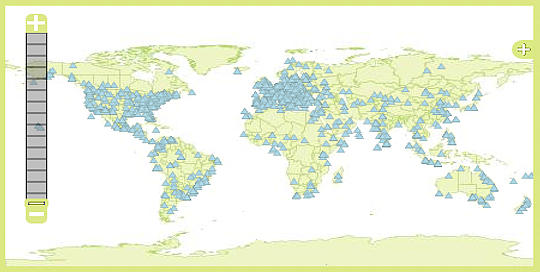
\includegraphics[clip=true, width=10cm]{community-map}
\end{center}
\end{figure}

With community platforms such as our website, wiki, forums and blog the QGIS project
provides current news, release, usage, and development information. In most cases 
these community web sites permit user contributions after registering. 
The QGIS-user mailing, forum and Internet Relay Chat (IRC) provide a valuable interface 
with other users and for discussions of QGIS in general. In the spirit of open 
process and sharing knowledge, contacting developers directly instead of going through 
these community based avenues of communication is frowned upon.

\subsection{Graphical User Interface}

Working with QGIS is simple and intuitive as you are presented with a
modern and friendly graphical user interface (GUI) based on QT4. All
functions are clearly separated (see Figure~\ref{fig:qgis10}).

\begin{figure}[h]
   \begin{center}
   \caption{Quantum GIS 1.0.0 'Kore'}\label{fig:qgis10}\smallskip
   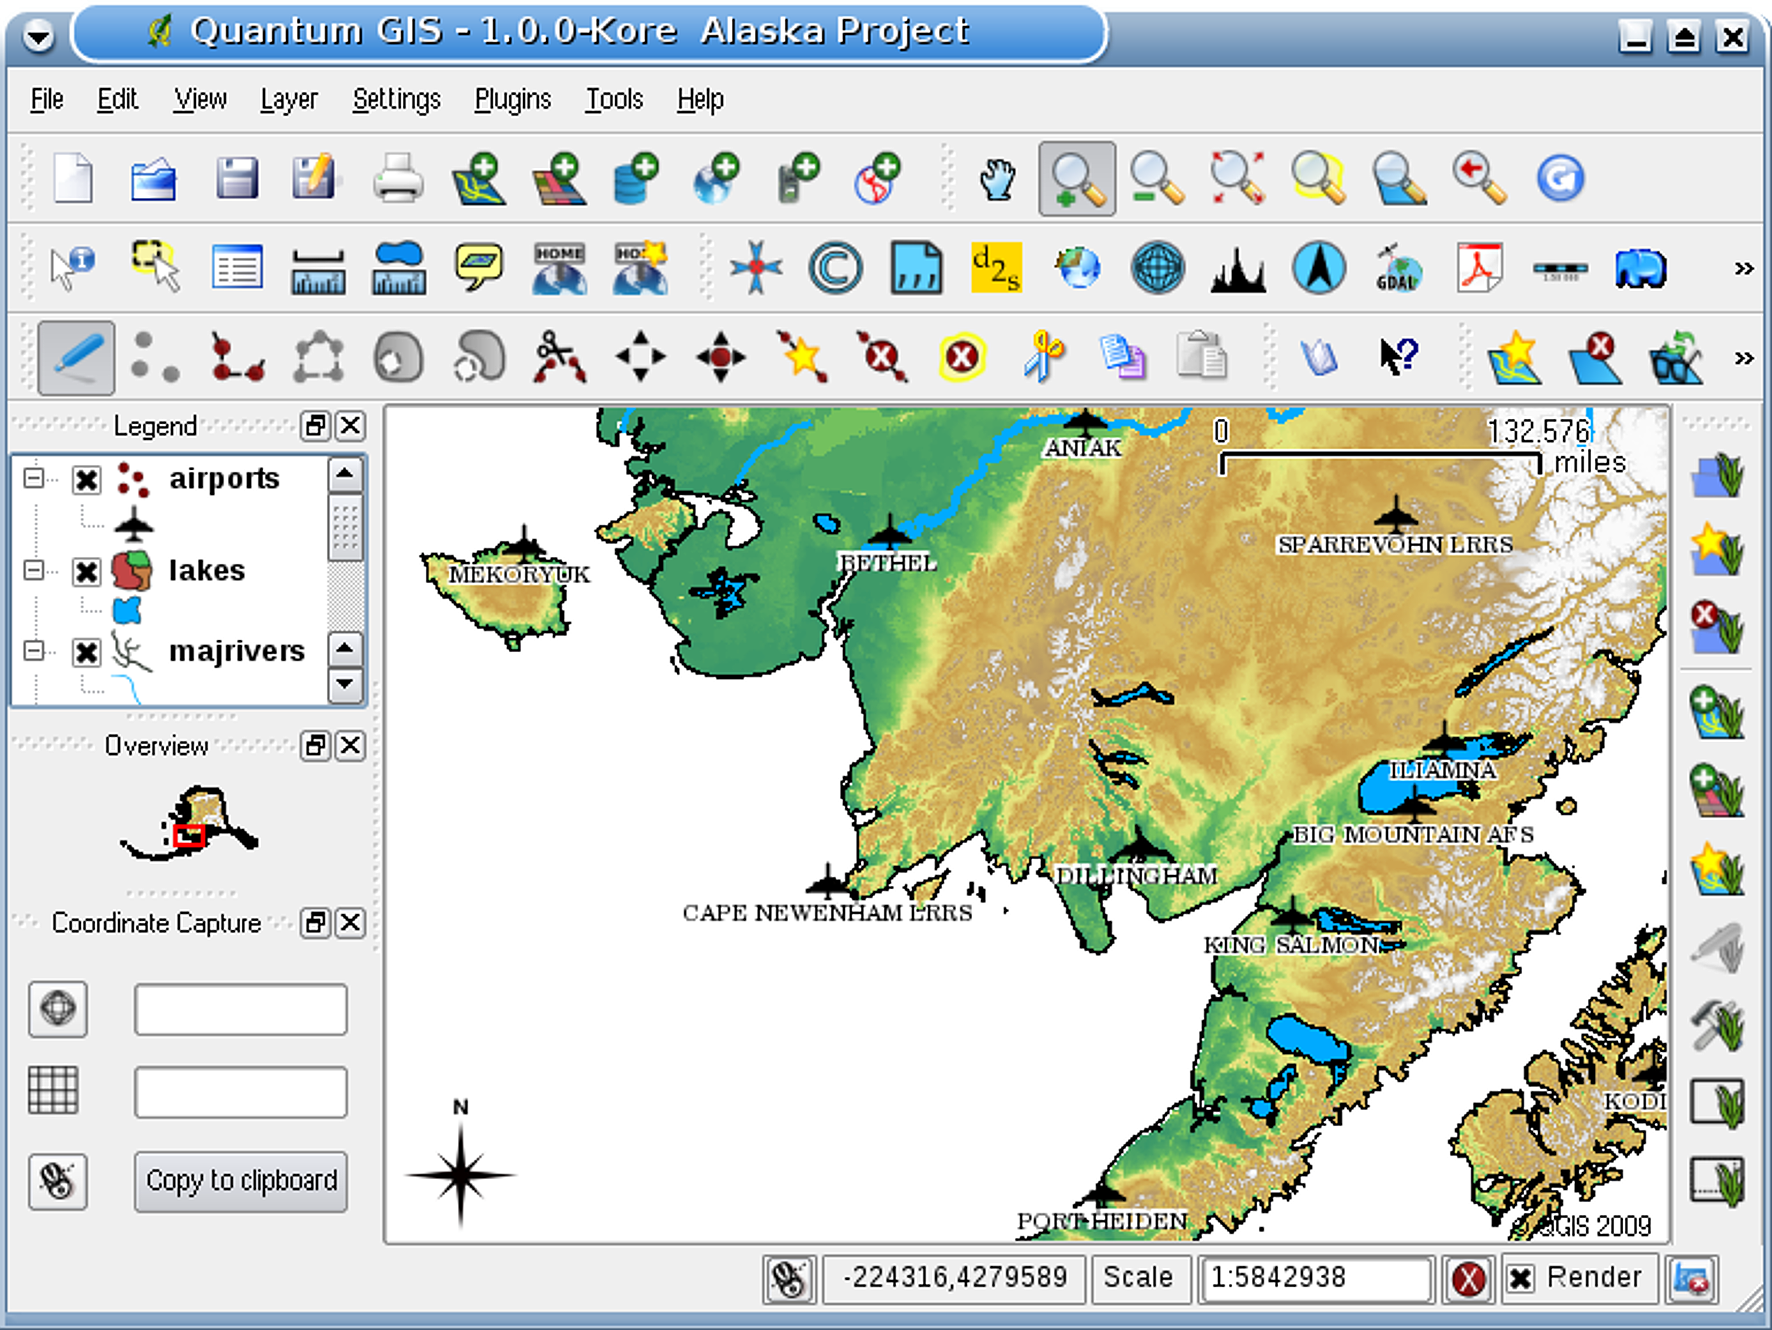
\includegraphics[clip=true, width=12cm]{qgis10}
\end{center}
\end{figure}

A \textbf{menu bar} provides access to QGIS features using a standard
hierarchical menu, with icons of the corresponding tools as they appear on
the tool bar and with keyboard shortcuts. The \textbf{tool bar} icons provide
direct access to functions of the menu bar, plus additional tools for
interacting with the map view. To make the GUI appear simpler, tool bar icons
can be switched on and off. The 'business end' of QGIS is the \textbf{map
view}. Various operations can be performed on the map, such as pan, zoom-in,
zoom-out, select or query. It is tightly bound to the \textbf{map legend},
where layer visibility is managed and set to a z-order, meaning layers
listed nearer the top of the legend are drawn over layers listed lower down.
The \textbf{map overview} area provides a full extent view of selected layers
with a rectangle showing the current map extent in the map view. And the
\textbf{status bar} finally shows the current mouse pointer position in map
coordinates, view extents of the map view, the progress of rendering or
analysis activities, the current map scale depending on the defined
Coordinate Reference System (CRS) and information about available external
plugin updates.

\subsection{Functionality}

QGIS offers a growing number of common GIS functionality provided by core
features and plugins and at a glance provide following features: 

\begin{itemize}
\item view and overlay vector and raster layer in different formats and
projections without conversion to an internal or common format. Supported are
PostgreSQL/PostGIS, GDAL/OGR supported vector and raster layers such as ESRI
Shapefile, MapInfo, GML, GeoTiff or Erdas Img., GRASS rasters, vectors, and locations, and
OGC-compliant WMS and WFS;
\item interactively explore data, including features such as on the fly
(OTF) projection, identify/select geometries, view, select and search
attributes, label features, change vector and raster symbology; 
\item compose print layouts adding map canvas, legend, scalebar, images and
text lables in a print composer plugin;
\item create, edit, manage and export vector layers into several formats.
Raster layer have to be imported into GRASS GIS to be edited and
exported;
\item perform spatial geoprocessing on PostgreSQL/PostGIS and other OGR
supported vector layers including overlay, buffer, sampling, geometry and
database management. The integrated GRASS Plugin allows to include the GRASS functionality of more than 300 modules.
\end{itemize}

\begin{figure}[h]
   \begin{center}
   \caption{QGIS Geoprocessing Tools}
    \label{fig:geoprocessing}\smallskip
   
\includegraphics[clip=true, width=8cm]{geoprocessing}
\end{center}
\end{figure}

\subsection{Plugin Architecture}

QGIS has been designed with a plugin architecture and therefore new
customised features and functions can easily be added to the application.
Many of the features in QGIS are actually implemented as core or external
plugins. 

\textbf{Core Plugins} are maintained by the QGIS Development Team. They are
written in C++ or Python, are automatically part of every QGIS distribution
and can be enabled with the Plugin Manager. There are currently 17 core
plugins available, including GRASS GIS integration (See
Figure~\ref{fig:grass-plugin}), Georeferencer, Mapserver Export, Shapefile to
PostGIS Import Tool, OGR Layer Converter, GPS Tools, Add Delimited Text Layer
and WFS support.

\begin{figure}[h]
   \begin{center}
   \caption{One of the QGIS Core Plugin (GRASS GIS Integration)}
    \label{fig:grass-plugin}\smallskip
   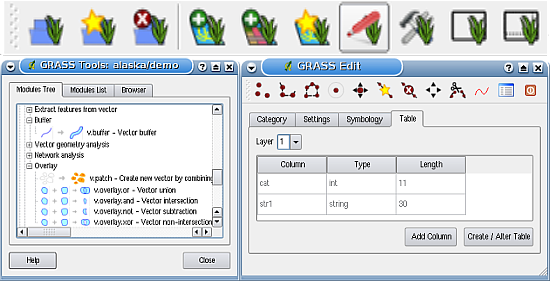
\includegraphics[clip=true, width=14cm]{grass-plugin}
\end{center}
\end{figure}

\textbf{External Plugins} are all written in Python and divided into official
and user contributed plugins. The user can easily add those Plugins to QGIS
with the Python Plugin Installer (See Figure~\ref{fig:python-plugin}).

\begin{itemize}
\item \textbf{Official} external python plugins are stored in an official,
moderated repository at \url{http://pyqgis.org/repo/official} as part of the
official QGIS release and maintained by their respective author.
\item \textbf{User-Contributed} external python plugins are stored in an
unofficial repository at \url{http://pyqgis.org/repo/contributed} and contain
plugins that are not yet mature enough but on the way to the official
repository.
\end{itemize}

Beside these two repositories a number of QGIS developers provide and maintain
their own repositories. These can be added to the repository list of the
Python Plugin Installer.

\begin{figure}[h]
   \begin{center}
   \caption{QGIS Python Plugin Installer}\label{fig:python-plugin}\smallskip
   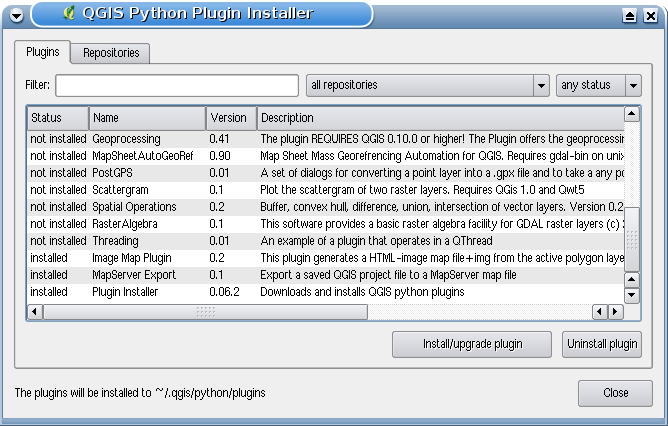
\includegraphics[clip=true, width=14cm]{python-plugin-installer}
\end{center}
\end{figure}

\subsection{Development}

%QGIS 1.0 provides a stable API from which custom solutions in Python or C++
%can be developed. Even though 1.0 is pretty fresh, there are already a number
%of exciting developments underway in both the core application and plugins.

Since QGIS is open source software, it is possible and encouraged to participate in the development
process and also to write new applications that use the libraries of the QGIS
project. Development with QGIS can be done either in the existing classes of
QGIS, as plugin extensions or in the form of custom applications that make use
of the QGIS libraries. All code in QGIS is licensed under the
GNU GPL (\url{http://www.fsf.org/licensing/licenses/gpl.html}). That means that for all three cases, published software must be
distributed under the terms of the GPL too. QGIS 1.0 provides a stable API which 
provides an assurance that plugins and applications developed against the 1.0 API 
will work against future releases in the 1.X release series.

\subsubsection{Development in the core classes of QGIS}
Changes to existing classes may be submitted as patches using QGIS Project bug
tracker (\url{https://trac.osgeo.org/qgis/}). The code maintainers of the QGIS
project, each responsible for a certain part of the code base, regularly check
the tracker.

\subsubsection{Development of extensions as C++ or Python plugins}
There is a plugin interface that allows extensions to access the running QGIS
instance and to use and extend the objects in the core of QGIS. Plugins may be
written in C++ or in Python. The QGIS documentation contains simple examples
for both programming languages making it straightforward to start with plugin 
programming. The development of python plugins is especially fast and convenient. Simple plugins require only a few hours of development. As a result, an increasing number of users are contributing new plugins, of either specialised or general use.

\subsubsection{Custom applications that use the QGIS libaries}
It is also possible to write new applications that provide their own user
interface and use the QGIS core library for the GIS logic, data access and map
rendering. 

An example using this approach is the QGIS mapserver project (\url{http://karlinapp.ethz.ch}) that provides a WMS
compatible mapserver on top of the QGIS core library. This software has no 
graphical user interface. It is a FastCGI application that waits until called
by a webserver. It parses the request parameters and uses QGIS to render a map
into an offscreen buffer. The content is then returned as binary image back to
the client.

Another context where this approach would make sense is to provide a mapping
application for mobile devices. Applications for mobile devices usually need
different user interfaces to desktop computers applications and
laptops. The QGIS libraries offer the potential to be used as a GIS backend for 
applications targeted to mobile devices.

\subsection{Who uses QGIS}
QGIS is now widely used by professionals, government and local agencies, universities and students, and amateurs alike, for a large variety of tasks, from simply viewing raster and vector data (especially useful is the capability to deal with PostGIS layers) to running complex and custom analyses through GRASS modules. Often is used to replace or integrate proprietary software, and several migrations have been accomplished or are underway, both in small and in large companies and public administrations. Among the hundreds of people that have attended courses on QGIS use, a common feeling is that the switch from proprietary software is painless, because many tasks and menus are very similar, and the interface is generally judged intuitive.

\subsection{Perspective / Conclusion}

\minisec{Authors}

The authors of this article are QGIS Project Steering Committee Members:

Otto Dassau <dassau@nature-consult.de>  
\\Gary Sherman <sherman@mrcc.com>
\\Tim Sutton <tim@linfiniti.com>
\\Marco Hugentobler <marco.hugentobler@karto.baug.ethz.ch>
\\Paolo Cavallini <cavallini@faunalia.it>

\minisec{Links}

For more information, have a look at the following website:

Quantum GIS project: \url{http://qgis.org}
\\QGIS Forum: \url{http://forum.qgis.org}
\\QGIS Blog: \url{http://blog.qgis.org}
\\QGIS User Mailing List: \url{http://lists.osgeo.org/mailman/listinfo/qgis-user}
\\QGIS IRC: Channel \#qgis port 6667 at \url{irc.freenode.net}
\\Open Source Geospatial Foundation: \url{http://www.osgeo.org}



